% Many thanks to Andrew West for writing most of this file
% Main LaTeX file for CIS400/401 Project Proposal Specification
%
% Once built and in PDF form this document outlines the format of a
% project proposal. However, in raw (.tex) form, we also try to
% comment on some basic LaTeX technique. This is not intended to be a
% LaTeX tutorial, instead just (1) a use-case thereof, and (2) a
% template for your own writing.

% Ordinarily we'd begin by specifying some broad document properties
% like font-size, page-size, margins, etc. -- We have done this (and
% much more) for you by creating a 'style file', which the
% 'documentclass' command references.
\documentclass{sig-alternate}
 
% These 'usepackage' commands are a way of importing additional LaTeX
% styles and formattings that aren't part of the 'standard library'
\usepackage{mdwlist}
\usepackage{url}
\usepackage{tabularx}
\usepackage{tikz}
\usepackage{mathbbol}
\usetikzlibrary{shapes,arrows}
\usepackage[export]{adjustbox}
\usepackage{lipsum,adjustbox}
\usepackage{listings}% http://ctan.org/pkg/listings
\DeclareMathSymbol{\fcmp}{\mathrel}{bbold}{\lq\;}
\lstset{
  basicstyle=\ttfamily,
  mathescape
}\begin{document} 


% We setup the parameters to our title header before 'making' it. Note
% that your proposals should have actual titles, not the generic one
% we have here.
\title{Verification of System FC in Coq}
\subtitle{Dept. of CIS - Senior Design 2014-2015\thanks{Advisors: Stephanie Weirich (sweirich@cis.upenn.edu), Richard Eisenberg (eir@cis.upenn.edu).}}
\numberofauthors{4}
\author{
  Tiernan Garsys \\ \email{tgarsys@seas.upenn.edu} \\ Univ. of Pennsylvania \\ Philadelphia, PA\\\\
  Lucas Pe\~{n}a \\ \email{lpena@seas.upenn.edu} \\ Univ. of Pennsylvania \\ Philadelphia, PA
  \and
  Tayler Mandel \\ \email{tmandel@seas.upenn.edu} \\ Univ. of Pennsylvania \\ Philadelphia, PA\\\\
  Noam Zilberstein \\ \email{noamz@seas.upenn.edu} \\ Univ. of Pennsylvania \\ Philadelphia, PA
}
\date{}
\maketitle

% Next we write out our abstract -- generally a two paragraph maximum,
% executive summary of the motivation and contributions of the work.
\begin{abstract}
\textit{
Haskell is a statically-typed functional programming language that is commonly used for the robust compile-time guarantees provided by its type system. Despite this usage, the type safety of Haskell has not been mechanically proven; it may be possible to write Haskell programs that type-check at compile-time but fall into an inconsistent state at runtime. Many safety critical systems such as flight controllers, self driving cars, and missile controllers are powered by software. If the type systems underlying this code are not verified, then the code itself is unsafe.
}

\textit{
This work approaches this problem by verifying System FC, the formalization of the core language of the Haskell compiler. It presents a mechanized proof for a large subset of System FC using the Coq Proof Assistant.  The type system of System FC is the basis for the type system of Haskell, so the results translate directly into safety guarantees at the program level.
}
\end{abstract}

% Then we proceed into the body of the report itself. The effect of
% the 'section' command is obvious, but also notice 'label'. Its good
% practice to label every (sub)-section, graph, equation etc. -- this
% gives us a way to dynamically reference it later in the text via the
% 'ref' command, e.g., instead of writing `Section 1', you can write
% `Section~\ref{sec:intro}', which is useful if the section number
% changes.

\section{Introduction}
\label{sec:intro}


Content content content

\section{Background}
\label{sec:background}

\subsection{Haskell}
\label{sec:background-haskell}

Haskell is a functional programming language originally released in 1990. Haskell is a statically-typed language; the types of all expressions and variables are determined at compile-time via either type inference or explicit type annotations by the programmer. Haskell is strongly-typed, meaning that the usage of values in identifier declarations and functions must be consistent with the statically-declared types of these functions; Haskell will not implicitly convert values from one type to another in order to satisfy the static typing of the program. Haskell is also a purely-functional language; a function defined in Haskell is guaranteed not to have side-effects such as I/O or the mutation of data structures in the running environment unless this is explictly allowed by the programmer. 

The strong static typing of Haskell is attractive because it allows the programmer to make certain guarantees about the properties of his or her program at compilation, rather than runtime. Such guarantees include the guarantee that a function is never called with an invalid input type, or the guarantee that a function defines a behavior for null inputs. By determining these properties at compile-time, one can rule out entire classes of errors prior to ever running the program.

These advantages are founded on the believed type safety of Haskell. Type safety in a programming language refers to its resilience to type errors at runtime. In the context of a statically-typed language such as Haskell, type safety requires ensuring that the guarantees of behavior made at compile-time are preserved during program execution. Given type safety, one can be sure that the program does not exhibit undefined behavior (such as segmentation faults) during execution.

\subsection{GHC Core}
\label{sec:background-ghc-core}

The Glasgow Haskell Compiler, or GHC, is an optimizing compiler used to generate native executables from Haskell code. As with most compilers, GHC compiles programs in multiple phases, translating the source between various intermediate representations. These phases of compilation are outlined in Figure~\ref{fig:desgar}. Whereas a surface language, such as Haskell, is structured to be easy for humans to work with, these intermediate representations (also known as {\em core languages}) are designed to be easy for a compiler to modify and optimize.

In the first phase of compilation, Haskell code is type-checked and then converted into a desugared intermediate language called GHC Core. The conversion from Haskell to GHC Core involves adding explicit type annotations to all values (which, in Haskell, can be omitted by the programmer and subsequently inferred when type-checking), adding explicit type parameters to type declarations with polymorphic types, and assigning all identifiers globally-unique names. Once converted, GHC performs optimizations on the resulting GHC Core code before passing the program on to later stages of compilation.

\begin{figure}[h!]
  \centering
  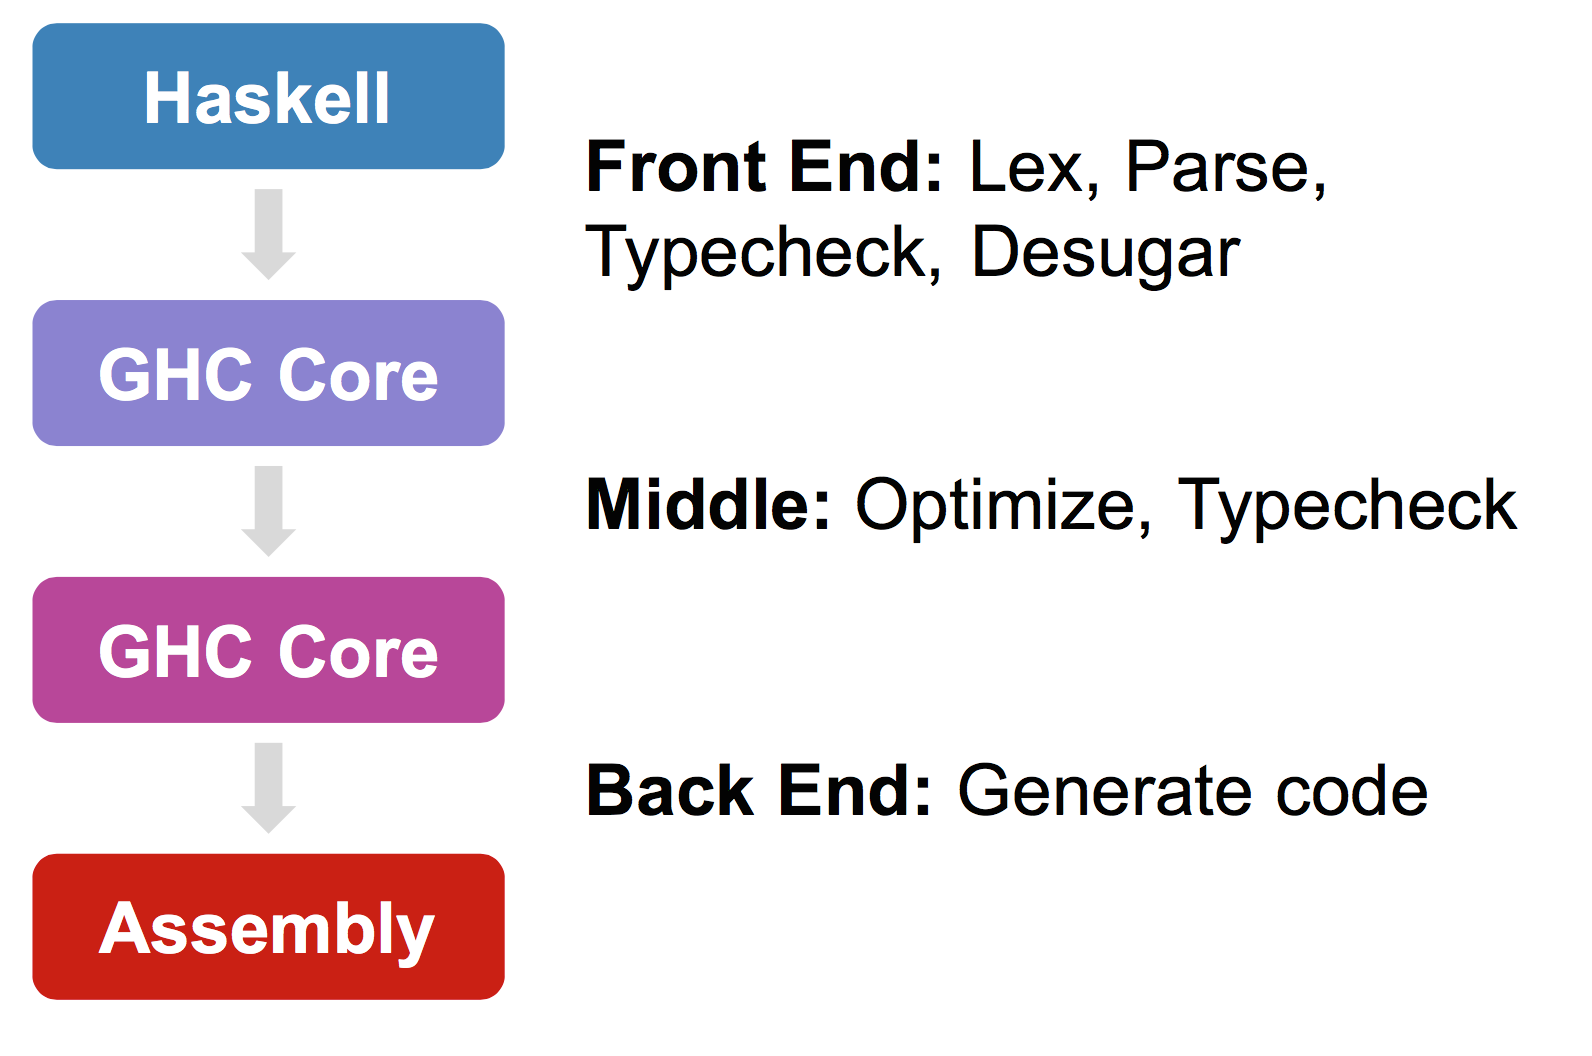
\includegraphics[max width=3in]{desgar.png}
  \caption{The GHC compilation process}
  \label{fig:desgar}
\end{figure}


\subsection{System FC}
\label{sec:background-fc}

GHC Core is an implementation of System FC, a formal language specification designed for use as an intermediate representation during the compilation of Haskell code \cite{conf/tldi/SulzmannCJD07}. The theoretical foundation of System FC is the untyped lambda calculus, a formal language used to express computations. The untyped lambda calculus builds up computations in terms of functions, allowing for one to construct function abstractions (which define a function in terms of some input variable) and function applications (which take an input argument and substitute instances of the function's input variable with that argument). From its small core, one can extend the untyped lambda calculus with additional features which may be useful in studying features of a language implementing an equivalent type system. One of the most widely-known extensions to the untyped lambda calculus is the simply-typed lambda calculus. This system is similar to the untyped lambda calculus, but adds the annotation of types to the arguments of functions. Whereas any value may be passed as an argument to a function in the untyped lambda calculus, an expression is only valid in the simply-typed lambda calculus if the type of an expression passed as an argument to a function is the same as the type annotation for that variable. This typing system is further extended by System F, also known as the polymorphic lambda calculus. In this system, the direct precursor to System FC, the simply-typed lambda calculus is extended with the ability to express universally quantified types. Universally quantified types are types which are parametrized by other types: for example, System F allows one to express a type $\Lambda\alpha.\alpha\rightarrow\alpha$, which is the type of a function which takes an input type $\alpha$ and a single expression of type $\alpha$ and returns an expression of type $\alpha$. This feature essentially allows for functions to take types as parameters, granting the ability to define functions whose actual types vary based on these input types, which can be useful in modeling surface language features such as parametric polymorphism or generics. 

System FC is a programming language specification defined in 2007 as a superset of the features present in System F \cite{conf/tldi/SulzmannCJD07}. System FC was introduced due to perceived shortcomings in System F as an intermediate language specification in GHC. While System F used to be sufficient as an intermediate representation for Haskell code, language designers have started experimenting with novel type systems such as generalized algebraic datatypes (or GADTs) and associated types that are either difficult or impossible to represent in System F. System FC ameliorates these issues by introducing features such as type coercions, type families, and datatypes. 
Type coercions allow for type families and generalized algebraic datatypes to exist in System FC by acting as a witness for equality between syntactically different types~\cite{DBLP:conf/rta/VytiniotisJ13}. For an example of coercions, see Figure 4. Types can be equal in different ways and therefore there is a complex set of coercion rules that can be used to construct correct equality proofs~\cite{Breitner:2014:SZC:2628136.2628141}. These equality proofs are responsible for most of the power of System FC over System F. They allow a conversion from one type to another. A basic example of the usefulness of coercions is provided in Figure 4.
\begin{verbatim}
data G a where
  G1 :: G Int
  G2 :: G Bool

f :: G a -> a
f G1 = 5
f G2 = True
\end{verbatim}
\begin{center}
\it Figure 4a: Haskell code where coercion is needed
\end{center}


\begin{lstlisting}
G :: * $\rightarrow$ *
G1 :: $\forall$ (a :: *). a $\sim$ Int $\rightarrow$ G a
G2 :: $\forall$ (a :: *). a $\sim$ Bool $\rightarrow$ G a

f :: $\forall$ (a :: *). G a $\rightarrow$ a
f = $\lambda$(a :: *). $\lambda$(x :: G a)
  case x of
    G1 c $\rightarrow$ 5 $\triangleright$ sym c
    G2 c $\rightarrow$ True $\triangleright$ sym c
\end{lstlisting}
\begin{center}
\it Figure 4b: Translation of Haskell code in Figure 4a to System FC. The necessity of is demonstrated here.
\end{center}

This is a basic example of datatypes in Haskell and a trivial use of them. \texttt{G} is a parameterized datatype with kind {\tt *} $\rightarrow$ {\tt *}. A \textit{kind} in Haskell represents the type of a type constructor. In Haskell, the types \texttt{Int} and \texttt{Bool} both have kind \texttt{*}. \texttt{f} is a function that takes something of type \texttt{G a} and returns something of type \texttt{a}. In Haskell, this only compiles because of coercions.

Here, \texttt{G1} is stating that for all types \texttt{a} of kind \texttt{*}, if \texttt{a} can be coerced to an \texttt{Int}, then one can obtain something of type \texttt{G a}. \texttt{G2} is defined similarly. Now, in the \texttt{G1} case, in order for the function \texttt{f} to correctly yield something of type \texttt{a}, \texttt{5} needs to be coerced to be of type \texttt{a}. This is accomplished using the rule from the construction of \texttt{G1}, since \texttt{G1} requires that an \texttt{a} can be coerced to an \texttt{Int}. The symmetry of this rule allows for \texttt{5} to be coerced to an \texttt{a}, which is required in the body of \texttt{f}. 

\subsection{Type Safety}
\label{sec:background-type-safety}

Types are used in programming languages as a means of classifying pieces of data; common examples of types include integers, characters, and boolean values. Types are used to determine guidelines for how one may work with a piece of data, such as the range of values that the data may take or the operations that are allowed to be performed with a given piece of data. By explicitly forming rules about how one may work with various pieces of data in a program, one has a powerful means of detecting and preventing program errors; attempting to operate on a piece of data in a way that is inconsistent with its typing will result in a type error, rather than simply performing some undefined operations [BEFORE THIS IS A BIT KLUDGY, AFTER THIS COULD PROBABLY BE EXPANDED]. Where these type errors occur is a language design choice that falls on a spectrum between dynamic typing and static typing. In dynamically-typed languages such as Python or JavaScript, judgments about whether an operation is well-typed are made during a program's execution. In constrast, statically-typed languages such as Haskell or OCaml determine whether operations are well-typed at compilation, with the expectation that these operations remain well-typed during execution. In practice, many statically-typed languages provide mechanisms by which the typing guarantees made at compile-time can be subverted. One common mechanism for this is runtime casting, which allows a programmer to assert that a value at a particular point of program execution may be treated as having a particular type different from that which can be guaranteed statically. In weighing the type safety of a language, it is common practice to focus on \"safe\" subsets of the language that omit such features. [LAST THREE SENTENCES NEEDED?]

Type safety, broadly, refers to the resiliency of a programming language to type errors over the course of executing a program in that language. In the context of statically-typed languages, type safety is achieved by ensuring that the program written in the language cannot enter an ill-typed (commonly referred to as {\em stuck}) state during execution. A stuck program is one that has finished evaluating to its final result, but has no way to continue execution as defined by the typing and evaluation semantics of the language. In a stuck state, the behavior of the program if one attempts to continue execution is undefined. In practice, hitting stuck states during execution might result in segmentation faults or the silent corruption of the program's state.

Proving that a language's typing and evaluation semantics exclude the possibility of reaching a stuck state is also referred to as proving the {\em soundness} of the language's type system. One strategy for proving the soundness of a language is to prove that the the theorems of Progress and Preservation hold for the language. [CAPITALIZE PROGRESS AND PRESERVATION?] {\em Progress}, at a high-level, states that the well-typedness of a program at some point in execution implies that the program may continue to be evaluated. {\em Preservation} states that the execution semantics of the language do not change the typing of the program; the typing for the program and its sub-components at any point in execution is consistent with that determined prior to execution. Soundness arises from these two theorems; if the language's execution semantics always have a defined behavior for a well-typed program and the well-typedness of a program is always preserved during the course of execution, then one knows that a well-typed program will always have a defined execution behavior. The exact formulation of these theorems for a language is dependent on how the evaluation and typing semantics are modeled by the verifier.


\section{Motivation}
\label{sec:motivation}

The primary motivation for this project is verify that the type safety guarantees provided by Haskell are actually well-founded. Haskell has found widespread usage due to the belief that its strong type system

Demonstrating the efficacy of Haskell's type system could also help to increase its adoption in critical systems, which could help to prevent catastrophic failures of these systems. Two recent software flaws which could have potentially been prevented through the use of type safe languages were the Shellshock and Heartbleed bugs.

This work is also motivated by the future extensions that can be made to the proofs. One area of direct extension is in proving that language extensions made to System FC in order to support new features in Haskell are type safe. Providing formal proofs of such features becomes increasingly relevant as the scope and complexity of System FC (and thus, the potential for errors in its formulation and verification) increases. Another area of direct extension for these proofs is in proving that the safety of various compiler optimizations, which risk changing the evaluation semantics of a given piece of code.

\section{Related Work}
\label{sec:related-work}

Content content content

\section{System Model}
\label{sec:model}
At a high-level, the system is composed of a formalization of the semantics of System FC, and a series of proofs of the properties of this formalization. The formalization itself is a representation of the System FC language using the language features of Coq. This is accomplished by defining inductive datatypes to serve as Coq correlates to the types (universally quantified types, function types, etc.) and terms (variables, type abstractions, etc.) introduced in System FC.  With these, one can in theory construct a representation of any System FC program. Actually modeling the execution of this is accomplished by translating the execution semantics of System FC to Coq. This is done by creating in Coq a series of relations and fixpoints (the Coq terminology for a function, like those defined in Haskell or OCaml) that map terms to terms and types to terms according to the execution rules of System FC. With this formalization of the execution semantics, one is able to create a representation of any System FC program and then simulate its execution in the context of Coq. More importantly, the complete formalization of the operational semantics for System FC allows for proofs to be written in Coq about these operational semantics which are essential to mechanically demonstrating the type soundness of System FC.

\section{Implementation}
\label{sec:implementation}

The proof is implemented using the Coq Proof Assistant. First, the language semantics are formalized in the Coq language and then the key theorems are proven based on this formalization. The main theorems are the Progress, Preservation, and Soundness theorems.

\subsection{Formalization}
\label{sec:implementation-formalization}

The formalization of System F in Coq follows directly from the definitions in~\cite{Pierce:TAPL}. The formalization of coercions comes from~\cite{Breitner:2014:SZC:2628136.2628141} and~\cite{DBLP:conf/tldi/YorgeyWCJVM12}. First, types, coercions, terms, and values are defined as inductive datatypes. Inductive datatypes are datatypes over which Coq can perform inductive proofs. This property is quite useful when proving the Progress and Preservation theorems. The formalization of System F syntax is shown in Figure~\ref{fig:syntax-coq} where \texttt{tm} represents a System FC term,  \texttt{ty} represents a System FC type, and \texttt{cn} represents a System FC coercion.

\begin{figure}[h!]
\begin{tabular}{lcll}
$t$ & $::=$ & & \textbf{Terms} \\
    & $|$   & $x$ & {\small Variables} \\
    & $|$   & $\lambda x:\tau.t$ & {\small Term Abstraction} \\
    & $|$   & $t_1\; t_2$ & {\small Term Application} \\
    & $|$   & $\Lambda \alpha.t$ & {\small Type Abstraction} \\
    & $|$   & $t\; \tau$ & {\small Type Application} \\
    & $|$   & $\lambda c:\varphi.t$ & {\small Coercion Abstraction} \\
    & $|$   & $t\; \gamma$ & {\small Coercion Application} \\
    & $|$   & $t \triangleright \gamma$ & {\small Safe Casting} \\
&&\; \hspace{.75in} \;& \\
$\Gamma$ & $::=$ & & \textbf{Contexts} \\
         & $|$   & $\varnothing$ & {\small Empty Context} \\
         & $|$   & $\Gamma,\; x:\tau$ & {\small Term Variable Binding} \\
         & $|$   & $\Gamma,\; \alpha$ & {\small Type Variable Binding} \\
         & $|$   & $\Gamma,\; c:\varphi$ & {\small Coercion Variable Binding}
\end{tabular}
\caption{System FC term and context syntax}
\label{fig:syntax-tex}
\end{figure}

\begin{figure}[h!]
\begin{tabular}{lcll}
$\tau$ & $::=$ & & \textbf{Types} \\
       & $|$   & $\alpha$ & {\small Variables} \\
       & $|$   & $\forall \alpha.\tau$ & {\small Polymorphic Types} \\
       & $|$   & $(\sigma_1 \sim \sigma_2) \Rightarrow \tau$ & {\small Coercion Polymorphism} \\
       & $|$   & $\tau_1 \rightarrow \tau_2$ & {\small Arrows} \\
&&\; \hspace{.75in} \;& \\
$\gamma$ & $::=$ & & \textbf{Coercions} \\
         & $|$   & $c$ & {\small Variables} \\
         & $|$   & $\langle\tau\rangle$ & {\small Reflexivity} \\
         & $|$   & $\textbf{sym}\gamma$ & {\small Symmetry} \\
         & $|$   & $\gamma_1 \fcmp\gamma_2$ & {\small Transitivity} \\
         & $|$   & $\gamma_1 \rightarrow\gamma_2$ & {\small Arrows} \\
         & $|$   & $\forall \alpha.\gamma$ & {\small Type Polymorphism} \\
         & $|$   & $(\gamma_1\sim\gamma_2)\Rightarrow\gamma$ & {\small Coercion Polymorphism} \\
         & $|$   & $\textbf{nth}^i\gamma$ & {\small Nth Argument Projection} \\
         & $|$   & $\gamma_1\; [\gamma_2]$ & {\small Instantiation} \\
\end{tabular}
\caption{System FC type and coercion syntax}
\label{fig:type-syntax}
\end{figure}

\begin{figure}[h!]
\begin{tabular}{cl}
\multicolumn{1}{l}{$\boxed{\vdash\Gamma}$} & \textbf{Well Formed Contexts} \\\\
\begin{tabular}{c}
  \hline
  $\vdash\varnothing$
\end{tabular} & {\small Empty Context} \\\\
\begin{tabular}{c}
  $\vdash\Gamma \;\;\;\; \Gamma \vdash \tau$ \\
  \hline
  $\vdash\Gamma,x:\tau$
\end{tabular} & {\small Term Variable Binding} \\\\
\begin{tabular}{c}
  $\vdash \Gamma$ \\
  \hline
  $\vdash\Gamma,\alpha$
\end{tabular} & {\small Type Variable Bindings} \\\\
\begin{tabular}{c}
  $\vdash\Gamma \;\;\;\; \Gamma\vdash\sigma_1 \;\;\;\; \Gamma\vdash\sigma_2$ \\
  \hline
  $\vdash\Gamma,c:(\sigma_1\sim\sigma_2)$
\end{tabular} & {\small Coercion Variable Bindings} \\
\; \hspace{.75in} \;& \\
\multicolumn{1}{l}{$\boxed{\Gamma \vdash \tau}$} & \textbf{Well Formed Types} \\\\
\begin{tabular}{c}
  $\alpha \in \Gamma$ \\
  \hline
  $\Gamma\vdash\alpha$
\end{tabular} & {\small Type Variables} \\\\
\begin{tabular}{c}
  $\Gamma\vdash\tau_1 \;\;\;\; \Gamma\vdash\tau_2$ \\
  \hline
  $\Gamma\vdash \tau_1\rightarrow\tau_2$
\end{tabular} & {\small Arrows} \\\\
\begin{tabular}{c}
  $\Gamma, \alpha\vdash \tau$ \\
  \hline
  $\Gamma\vdash \forall\alpha.\tau$
\end{tabular} & {\small Polymorphic Types} \\\\
\begin{tabular}{c}
  $\Gamma\vdash\sigma_1 \;\;\;\; \Gamma\vdash\sigma_2 \;\;\;\; \Gamma\vdash\tau$ \\
  \hline
  $\Gamma\vdash (\sigma_1\sim\sigma_2)\Rightarrow\tau$
\end{tabular} & {\small Coercion Polymorphism} \\
\end{tabular}
\caption{System FC well-formedness rules for contexts and types}
\label{fig:type-syntax}
\end{figure}


\begin{figure}[h!]
\begin{tabular}{cl}
\multicolumn{1}{l}{$\boxed{\Gamma \vdash \gamma : \varphi}$} & \textbf{Coercion Typing} \\\\
\begin{tabular}{c}
  $\vdash\Gamma \;\;\;\; c : \varphi \in \Gamma$ \\
  \hline
  $\Gamma\vdash c : \varphi$
\end{tabular} & {\small Coercion Variables} \\\\
\begin{tabular}{c}
  $\vdash\Gamma \;\;\;\; \Gamma\vdash\tau$ \\
  \hline
  $\Gamma\vdash \langle\tau\rangle : \tau\sim\tau$
\end{tabular} & {\small Reflexivity} \\\\
\begin{tabular}{c}
  $\Gamma\vdash \gamma : \sigma_1\sim\sigma_2$ \\
  \hline
  $\Gamma\vdash \textbf{sym}\gamma : \sigma_2\sim\sigma_1$
\end{tabular} & {\small Symmetry} \\\\
\begin{tabular}{c}
  $\Gamma\vdash\gamma_1 : \sigma_1\sim\sigma_2$ \\
  $\Gamma\vdash\gamma_2 : \sigma_2\sim\sigma_3$ \\
  \hline
  $\Gamma\vdash \gamma_1\fcmp\gamma_2 : \sigma_1\sim\sigma_3$
\end{tabular} & {\small Transitivity} \\\\
%% \begin{tabular}{c}
%%   $\Gamma\vdash\gamma_1 : \sigma_1\sim\sigma_2$ \\
%%   $\Gamma\vdash\gamma_2 : \tau_1\sim\tau_2$ \\
%%   \hline
%%   $\Gamma\vdash \gamma_1\rightarrow\gamma_2 : \sigma_1\rightarrow\tau_1\sim\sigma_2\rightarrow\tau_2$
%% \end{tabular} & {\small Arrows} \\\\
%% \begin{tabular}{c}
%%   $\Gamma\vdash\gamma : \sigma_1\sim\sigma_2$ \\
%%   \hline
%%   $\Gamma\vdash \forall\alpha.\gamma : \forall\alpha.\sigma_1 \sim \forall\alpha.\sigma_2$
%% \end{tabular} & {\small Type Polymorphism} \\\\
%% \begin{tabular}{c}
%%   $\Gamma\vdash\gamma_1 : \sigma_1\sim\tau_1$ \\
%%   $\Gamma\vdash\gamma_2 : \sigma_2\sim\tau_2$ \\
%%   $\Gamma\vdash\gamma_3 : \sigma_3\sim\tau_3$ \\
%%   \hline
%%   $\Gamma\vdash (\gamma_1\sim\gamma_2)\Rightarrow\gamma_3 : (\sigma_1\sim\sigma_2)\Rightarrow\sigma_3 \sim (\tau_1\sim\tau_2)\Rightarrow\tau_3$
%% \end{tabular} & {\small Coercion Polymorphism} \\\\
\begin{tabular}{c}
  $\Gamma\vdash\gamma_1 : \forall\alpha.\tau_1 \sim \forall\alpha.\tau_2$ \\
  $\Gamma\vdash\gamma_2 : \sigma_1   \sim \sigma_2$ \\
  \hline
  $\Gamma\vdash \gamma_1\;[\gamma_2] : \tau_1[\sigma_1/\alpha] \sim \tau_2[\sigma_2/\alpha]$
\end{tabular} & {\small Instantiation} \\\\
\end{tabular}
\caption{Selected System FC coercion typing rules}
\label{fig:coercion-typing}
\end{figure}


\begin{figure}[h!]
\begin{tabular}{cl}
\multicolumn{1}{l}{$\boxed{\Gamma \vdash t : \tau}$} & \textbf{Term Typing} \\\\
\begin{tabular}{c}
  $\vdash\Gamma \;\;\;\; x : \tau \in \Gamma$ \\
  \hline
  $\Gamma\vdash x : \tau$
\end{tabular} & {\small Variables} \\\\
\begin{tabular}{c}
  $\Gamma,x:\tau_1 \vdash t : \tau_2$ \\
  \hline
  $\Gamma\vdash \lambda x:\tau_1.t : \tau_1 \rightarrow\tau_2$
\end{tabular} & {\small Term Abstraction} \\\\
\begin{tabular}{c}
  $\Gamma\vdash t_1 : t_1\rightarrow t_2$ \\
  $\Gamma\vdash t_2 : t_1$ \\
  \hline
  $\Gamma\vdash t_1\; t_2 : \tau_2$
\end{tabular} & {\small Term Application} \\\\
\begin{tabular}{c}
  $\Gamma,\alpha:\sigma\vdash t_1 : t : \tau$ \\
  \hline
  $\Gamma\vdash \Lambda\alpha.t : \forall\alpha.\tau$
\end{tabular} & {\small Type Abstraction} \\\\
\begin{tabular}{c}
  $\vdash\Gamma \;\;\;\; \Gamma\vdash\tau$ \\
  $\Gamma\vdash t : \forall\alpha.\sigma$ \\
  \hline
  $\Gamma\vdash t\; [\sigma] : \tau[\sigma/\alpha]$
\end{tabular} & {\small Type Application} \\\\
\begin{tabular}{c}
  $\Gamma\vdash\varphi \;\;\;\; \Gamma,c:\varphi\vdash t : \tau$ \\
  $\Gamma\vdash t : \forall\alpha.\sigma$ \\
  \hline
  $\Gamma\vdash \lambda c:\varphi.t : \varphi\Rightarrow\tau$
\end{tabular} & {\small Coercion Abstraction} \\\\
\begin{tabular}{c}
  $\Gamma\vdash t : \varphi \Rightarrow \tau$ \\
  $\Gamma\vdash \gamma : \varphi$ \\
  \hline
  $\Gamma\vdash t\; \gamma : \tau$
\end{tabular} & {\small Coercion Application} \\\\
\begin{tabular}{c}
  $\Gamma\vdash \gamma : \tau_1\sim\tau_2$ \\
  $\Gamma\vdash t : \tau_1$ \\
  \hline
  $\Gamma\vdash t \triangleright \gamma : \tau_2$
\end{tabular} & {\small Safe Casting} \\\\

\end{tabular}
\caption{System FC term typing rules}
\label{fig:term-typing}
\end{figure}

\begin{figure}[h!]
\begin{tabular}{cl}
\multicolumn{1}{l}{$\boxed{t_1\longrightarrow t_2}$} & \textbf{One-Step Reduction} \\\\
\begin{tabular}{c}
  $t_1 \longrightarrow t'_2$ \\ 
  \hline
  $t_1\; t_2 \longrightarrow t'_1\; t_2$
\end{tabular} & {\small Term Reduction} \\\\
\begin{tabular}{c}
  \hline
  $(\lambda x:\tau.t)\; t' \longrightarrow t[t'/x]$
\end{tabular} & {\small Term Application} \\\\
\begin{tabular}{c}
  $t_1 \longrightarrow t'_2$ \\ 
  \hline
  $t_1\; [\tau] \longrightarrow t'_1\; [\tau]$
\end{tabular} & {\small Type Reduction} \\\\
\begin{tabular}{c}
  \hline
  $(\Lambda\alpha.t)\; [\tau] \longrightarrow t[\tau/\alpha]$
\end{tabular} & {\small Type Application} \\\\
\begin{tabular}{c}
  $t_1 \longrightarrow t'_2$ \\ 
  \hline
  $t_1\; \gamma \longrightarrow t'_1\; \gamma$
\end{tabular} & {\small Coercion Reduction} \\\\
\begin{tabular}{c}
  \hline
  $(\lambda c:\varphi.t)\; \gamma \longrightarrow t[\gamma/c]$
\end{tabular} & {\small Coercion Application} \\\\
\begin{tabular}{c}
  $t_1 \longrightarrow t'_2$ \\ 
  \hline
  $t_1 \triangleright \gamma \longrightarrow t'_1\triangleright \gamma$
\end{tabular} & {\small Casting Reduction} \\\\
\begin{tabular}{c}
  \hline
  $(t\triangleright\gamma_1) \triangleright\gamma_2 \longrightarrow t\triangleright \gamma_1\fcmp\gamma_2$
\end{tabular} & {\small Coercion Transitivity} \\\\
\begin{tabular}{c}
  $\varnothing\vdash v : \sigma_1 \rightarrow \sigma_2$ \\
  \hline
  $(v \triangleright \gamma) t \longrightarrow$ \\
  $v (t \triangleright \textbf{sym}(\textbf{nth}^1\gamma)) \triangleright \textbf{nth}^2\gamma$
\end{tabular} & {\small Term Application Push} \\\\
\begin{tabular}{c}
  $\varnothing\vdash v : \forall\alpha.\tau$ \\
  \hline
  $(v \triangleright \gamma)\; [\sigma] \longrightarrow v\; [\sigma] \triangleright \gamma\; [\sigma]$
\end{tabular} & {\small Type Application Push} \\\\
\begin{tabular}{c}
  $\gamma' = \textbf{nth}^1\gamma_0 \fcmp \gamma \fcmp \textbf{sym}(\textbf{nth}^2\gamma_0)$ \\
  $\varnothing\vdash v : (\sigma_1 \sim \sigma_2) \Rightarrow \tau$ \\
  \hline
  $(v \triangleright \gamma_0) \gamma \longrightarrow v\; \gamma' \triangleright \textbf{nth}^3\gamma_0$
\end{tabular} & {\small Coercion Application Push} \\\\
\end{tabular}
\caption{System FC evaluation rules}
\label{fig:evaluation}
\end{figure}


\begin{figure}[h!]
\begin{lstlisting}
(** *** Types *)
Inductive ty : Type := 
  | TVar    : nat -> ty 
  | TArrow  : ty -> ty -> ty
  | TUniv   : ty -> ty
  | TCoerce : ty -> ty -> ty -> ty.

(** *** Coercions *)

Inductive cn : Type :=
  | CVar     : nat -> cn
  | CRefl    : ty -> cn
  | CSym     : cn -> cn
  | CTrans   : cn -> cn -> cn
  | CArrow   : cn -> cn -> cn
  | CTCoerce : cn -> cn -> cn -> cn
  | CNth     : nat -> cn -> cn
  | CTAbs    : cn -> cn
  | CTApp    : cn -> ty -> cn.

(** *** Terms *)
Inductive tm : Type :=
  | tvar    : nat -> tm
  | tapp    : tm -> tm -> tm
  | tabs    : ty -> tm -> tm
  | ttapp   : tm -> ty -> tm
  | ttabs   : tm -> tm
  | tcapp   : tm -> cn -> tm
  | tcabs   : ty -> ty -> tm -> tm
  | tcoerce : tm -> cn -> tm.

(** *** Values *)
Inductive uncoerced_value : tm -> Prop :=
  | uv_abs : forall T t,
      uncoerced_value (tabs T t)
  | uv_tabs : forall t,
      uncoerced_value (ttabs t)
  | uv_cabs : forall t T1 T2,
      uncoerced_value (tcabs T1 T2 t).

Inductive value : tm -> Prop :=
  | v_uncoerced : forall t,
      uncoerced_value t ->
      value t
  | v_coerced : forall t c,
      uncoerced_value t ->
      value (tcoerce t c).

\end{lstlisting}
\caption{System FC syntax defined in Coq}
\label{fig:syntax-coq}
\end{figure}

In this formalization of the language, variables are parameterized by a natural number instead of a string as one would normally expect. Generally, variables are named with strings, but two different variables could share a name, which causes issues when reasoning about a language using Coq. Conflicting variable names creates a problem for handling shadowing and substitution. For example, when given a function $(\lambda x:Int.\:x + y)$ and attempting to substitute some externally defined variable $x$ for all instances of $y$, problems arise. Performing a na\"ive substitution of $[y \mapsto x] (\lambda x:Int.\:x + y)$ results in a function $\lambda x:Int.\:x + x$. This changes how the function evaluates, so it does not preserve program semantics. Continuing without addressing this source of error in the specification of the operational semantics of the language would make proving the type system to be sound impossible.

There are several ways to get around this substitution issue. The way substitution is handled in the system described is through the use of De Bruijn indices~\cite{Vouillon12}. This means that variables are encoded with natural number values. The value represents the number of binders between the variable's use and its binding site. Given this representation of variables, there cannot be naming conflicts. Consider the following example:
$$\Lambda T.\:\Lambda U.\:\lambda f:T \rightarrow U.\:\lambda x:T.\:f\:x$$
which has type:
$$\forall T.\:\forall U.\:(T \rightarrow U) \rightarrow T \rightarrow U$$
Using De Bruijn indices for both types and terms, the expression becomes:
$$\Lambda.\:\Lambda.\:\lambda : 1 \rightarrow 0.\:\lambda : 1.\:\overline{1}\:\overline{0}$$
which has type:
$$\forall.\:\forall.\:(1 \rightarrow 0) \rightarrow 1 \rightarrow 0$$

Note that the above uses bars to describe identifiers for terms. The $0$ refers to the closest type variable binder and $\overline{0}$ refers to the closest term variable binder. The first expression with traditionally named variables is a simple pair of type abstractions containing a pair of term abstractions related to the types introduced in the outer type abstractions. The variables must be explicitly named at the binding site. This is noted by the $\Lambda T.$ or $\lambda x:T$. Using De Bruijn indices eliminates this need, as referring to a binder just requires determining the distance from the usage site to the binding site. The $\Lambda T.$ in the first example is replaced simply by $\Lambda.$ and the $\lambda x:T$ is transformed into $\lambda : 1$. This is more clear in Figure~\ref{fig:syntax-coq}, where \texttt{tabs} and \texttt{ttabs} are not bound with associated identifiers as they would be with named variables. The $1$ here replaces the $T$, as there is a single type variable binder between the usage of the type and the desired binder.

This representation of variable names using De Bruijn indices is noted in the formalization in Figure~\ref{fig:syntax-coq} in the variable cases in $ty$, $tm$, and $cn$. All of these definitions take in a natural number as the variable name. This formalization affects the proofs through the rest of the implementation, most notably introducing the need for index shifting. Take, for example, the substitution $[Y \mapsto X] (\Lambda X.\:X \rightarrow Y)$ where $X$ is to be substituted for $Y$ in the type abstraction. Using De Bruijn indices, assume the outer $X$ is known as $2$ and the outer $Y$ is known as $3$ outside of the lambda. If this were the case, then the inner $X$ would have to be $0$ using De Bruijn indices, as it refers to the closest binding lambda to it. The inner $Y$ would then refer to the same binder as the outer $Y$. Even though the outer $Y$ is known as $3$ outside of the type abstraction, it must be known as $4$ inside of the abstraction, as an extra binder is introduced between the two uses of $Y$. Despite the confusion this may introduce, this makes the substitution $[3 \mapsto 2] (\Lambda.\:0 \rightarrow 4)$. This is where shifting is relevant. A na\"ive substitution would look for all instances of $3$ and replace them with $2$. This is not correct, though, as the search for uses of $3$ passes a binding site for type variables as it enters the lambda. This means that what used to be $3$ binders away from the binding site is now $4$ away. Thusly, shifting the index of the substituted variables is necessary to preserve program semantics and adequately work toward a proof of the type safety of System FC.

In order to handle the several forms of substitutions that can occur in the language, substitution is defined as Coq Notation. Notation in Coq allows the user to refer to fixpoints (functions) and datatypes using operators instead of names. In this implementation, the notation for substitutions is \texttt{[x := s]t} meaning substitute the identifier \texttt{x} with \texttt{s} in \texttt{t}. There are a number of different types of substitutions that an occur in the language between all permutations of types, terms, and coercions, meaning that \texttt{s} and \texttt{t} are not always the same type. In order for the substitution notation to be be reusable for the different kinds of substitutions, there is a \texttt{Subst} typeclass that has instances for the combinations of types for \texttt{x}, \texttt{s}, and \texttt{t}. In addition to being defined using fixpoints, substitutions are defined inductively. Fixpoints provide a nice notation for substitutions while the inductive definition is useful in proofs. In order to reconcile this, several lemmata are proven that verify the equivalence between the fixpoint and inductive definitions for substitutions. This allows theorems to use the more readable notation, while the proofs of those theorems use the inductive definitions.

After formalizing syntax and substitutions for System FC, the evaluation semantics of System FC are then defined via the step relation. In order to ensure the safety of a type system, some formalization of how expressions in the language evaluate is needed to reason about the full execution of a program in the target language. The described formalization takes from the small-step language semantics in~\cite{Pierce:SF} to define how a single expression can take a single step toward its final value. This is defined inductively with the associated notation \texttt{t1 ==> t2} meaning that term \texttt{t1} steps to a term \texttt{t2}. [NOAM SHOULD INSERT RULES HERE].

Variable binding contexts are implemented as an inductive datatype where \texttt{empty} represents the empty context and the data constructors \texttt{ext\textunderscore var} and \texttt{ext\textunderscore tvar} extend a context with a term or type variable binding respectively. Since variables are identified by de Bruijn indices, there is no need to specify any kind of identifier when binding a variable. By definition, a variable with de Bruijn index $n$ is bound $n$ levels up from the current scope. This means that the binding is the $n^\text{th}$ deep type/term/coercion variable binding in the context \texttt{Gamma}~\cite{Vouillon12}.

With contexts defined, it is possible to define the final piece of the System FC formalization, typing. Typing is defined as an inductive proposition called \texttt{has\textunderscore type}. A notation is also defined for the typing relation: \texttt{Gamma |- t \textbackslash in T} means that the term \texttt{t} has type \texttt{T} under the context \texttt{Gamma}. Since the type of this expression in Coq is \texttt{Prop} (short for proposition), it is an expression that must be true if it can be proven in Coq. Given the formalization presented above, it is possible to prove that any well typed term \texttt{t} with type \texttt{T} indeed has type \texttt{T}. If \texttt{t} is not well-typed, then it is impossible to prove that it has any type.

\subsection{Progress}
\label{sec:implementation-progress}

The next step after fully formalizing System FC is to prove the Progress theorem. The formal definition of Progress in Coq can be seen in Figure~\ref{fig:progress-coq}. More intuitively, the Progress theorem states that any term that is well-typed under the empty context is either a value or it can take a step. The proof of progress is by induction on the typing derivation \texttt{empty |- t \textbackslash in T}. Recall that the \texttt{has\textunderscore type} relation is defined inductively, therefore it is possible to proceed with an inductive proof over the relation.

\begin{figure}[h!]
\begin{lstlisting}
Theorem progress : forall t T, 
     empty |- t \in T ->
     value t \/ exists t', t ==> t'.
\end{lstlisting}
\caption{The Progress Theorem written in Coq}
\label{fig:progress-coq}
\end{figure}

The proof is laid out so as to have a separate case for every constructor in the inductive definition of \texttt{has\textunderscore type}. The cases for the typing relations of values represent base cases in the inductive proof. In the other cases, Coq provides induction hypotheses that must be applied in order to complete the proof. Most of the cases can be automated by Coq; the goals are straightforward to prove. The most involved cases are term application, type application, and coercion application. These are more complicated because it is necessary to handle the sub-cases where the terms, types, or coercions in the application could be values or could step.

[ Push rules? ]

\subsection{Preservation}
\label{sec:implementation-preservation}

The proof of Preservation is significantly more involved than the proof of Progress. The formal definition of Progress in Coq can be seen in Figure~\ref{fig:preservation-coq}. The Preservation theorem states that any term will preserve its type when taking a step. If a term has type \texttt{T} and then takes a step, the resulting term will also have type \texttt{T}. 

\begin{figure}[h!]
\begin{lstlisting}
Theorem preservation : forall Gamma t t' T, 
    Gamma |- t \in T ->
    t ==> t'         ->
    Gamma |- t' \in T.
\end{lstlisting}
\caption{The Preservation Theorem written in Coq}
\label{fig:preservation-coq}
\end{figure}

Several lemmata must be proven before Preservation itself can be proven. Among these, several weakening and strengthening lemmata help one reason about the well-formedness of a context or a coercion with a variable extended or removed. Also included are several substitution lemmata which are used to prove that substituting a type, term, or coercion in an expression preserves the type of the expression. Using these lemmata, the Preservation theorem is also proven by induction on the typing derivation \texttt{Gamma |- t \textbackslash in T}. Much like the Progress theorem, the majority of the work done in the proof takes place in cases for term, type, and coercion application.

\subsection{Soundness}
\label{sec:implementation-soundness}

The final theorem in proving the type safety of System FC is the Soundness Theorem. The formal definition of Soundness in Coq can be seen in Figure~\ref{fig:soundness-coq}. This theorem states that at any point in a well-typed term's execution, after any number of discrete steps, the term will not be in a stuck state, where a stuck state is any state where the term is not a value but also cannot take a step. More explicitly, this theorem says that if the type checker considers a term well-typed, then it will never get stuck in some inconsistent state, which is one standard definition of type safety. The proof of the Soundness theorem is done by induction on the number of discrete steps taken and a straightforward application of the Progress and Preservation theorems.

\begin{figure}[h!]
\begin{lstlisting}
Theorem soundness : forall t t' T,
    empty |- t \in T ->
    t ==>* t'        ->
    ~(stuck t').
\end{lstlisting}
\caption{The Soundness Theorem written in Coq}
\label{fig:soundness-coq}
\end{figure}

\section{Results}
\label{sec:results}

The system as it stands is a full mechanical proof of the type safety of System F with coercions. The type safety of all features of System FC have previously been proven by hand [CITE THIS], though it has never been done mechanically using a proof assistant. The system described is the first mechanical proof of this particular subset of System FC, namely System F with coercions. Other mechanical proofs of the type safety of System F exist, though none contain a formalization of coercions as described in~\cite{Breitner:2014:SZC:2628136.2628141} and~\cite{DBLP:conf/tldi/YorgeyWCJVM12}.

[ This means that this formalization of coercions is type safe when added to System F ].

Given that the Coq interpreter has accepted the proof, it is thought to be verified as a proper proof. The benefits of a mechanical proof over a handwritten one are many in number. A mechanical proof makes use of the Curry-Howard isomorphism to verify the proof instead of relying on the writer and other human verifiers. Beyond just correctness, a mechanical proof is also highly extensible. The system itself is a first for this subset of System FC, but it also allows for further extension to a larger subset, moreso than a handwritten proof could. 

[ WHAT EVEN GOES IN THIS SECTION ]

\section{Future Work}
\label{sec:future-work}

As the formalization stands, it does not contain all features commonly thought to be part of System FC. In order to reach feature parity with the full System FC, it would need to be extended to include data types and type families. These two additions would create the full formalization of System FC. It would then be necessary to adjust the proofs accordingly so that the Coq interpreter would accept them. A proof of the type safety of this more complete version of System FC would be a big step toward a proof of the type safety of Haskell. Recall that System FC is a specification for GHC Core, the actual implementation used in GHC, so a correctness proof of the translation from System FC to GHC Core would be necessary to have a proof of the type safety of System FC as used in the Haskell compilation process.

The mechanical proof as it stands is very extensible. This allows for a large number of potential extensions and use cases. Modifying a mechanical proof can be done by adding to an already proper formalization and then walking through the proof with the help of the Coq interpreter to fix anything broken by the change to the formalization. Given that most of the proofs in the system are done by induction on some inductive definition in the formalization, adding to the formalization would in most cases only add new cases, and much of the proof structure and the correctness of many of the proofs would be preserved.

With a full formalization and proof of System FC, possible extensions include verifying the safety of various GHC language extensions. GHC includes many features, but programmers are given even more options via extensions to the language. These can be included by annotating the program or adding command-line flags. Many commonly used language extensions add to Haskell's type system, so being able to prove the type safety of an extension would allow for an added level of guarantees to the potentially unsafe extension.

A mechanical proof of the type safety of GHC Core could also be used to check properties of compiler optimizations. At the GHC Core stage of GHC's compilation process, GHC does many of its optimization passes. Using the formalization and proof of type safety, one could extend the formalization to include a set of compiler optimizations. These optimizations could then be proven to be type safe to ensure the semantics of a program cannot be changed through an invalid optimization done at the GHC Core level.

\section{Ethics}
\label{sec:ethics}

As discussed above, one of the primary areas of future work with this formalization is using it as the foundation for future verification of optimizations and language extensions. These use cases raise the concern that the presented formalizations and thus presented proofs are incorrect. In the case where this work were to falsely suggest that System FC is type-safe, one would be left with the concern that numerous language extensions, compiler systems, and software systems were constructed on the false premise that their underlying type system was not inherently flawed. The real-world impact of these flaws is dependent on how likely it is for runtime systems to reach an inconsistent state in the flawed type system and how critical the systems that demonstrate these flaws are. 

Another potential issue arises in the case where this work were to falsely suggest that System FC is not type-safe. This would present a major breach of the trust people place in programming languages such as Haskell that are reliant on System FC, potentially leading to the adoption of less safe languages for critical systems.

MAKE PARAGRAPHS BECAUSE THIS IS VERY SENSATIONALISTIC AND PRETTY BAD

\section{Conclusion}
\label{sec:conclusion}

Content content content

% We next move onto the bibliography.
\bibliographystyle{plain} % Please do not change the bib-style
\bibliography{final_report}  % Just the *.BIB filename

% Here is a dirty hack. We insert so much vertical space that the
% appendices, which want to begin in the left colunm underneath
% "references", are pushed over to the right-hand column. If we looked
% hard enough, there is probably a command to do exactly this (and
% wouldn't need tweaked after edits).
\vspace{175pt}

\end{document} 
